% Options for packages loaded elsewhere
\PassOptionsToPackage{unicode}{hyperref}
\PassOptionsToPackage{hyphens}{url}
\PassOptionsToPackage{dvipsnames,svgnames,x11names}{xcolor}
%
\documentclass[
  letterpaper,
  DIV=11,
  numbers=noendperiod,
  oneside]{scrreprt}

\usepackage{amsmath,amssymb}
\usepackage{iftex}
\ifPDFTeX
  \usepackage[T1]{fontenc}
  \usepackage[utf8]{inputenc}
  \usepackage{textcomp} % provide euro and other symbols
\else % if luatex or xetex
  \usepackage{unicode-math}
  \defaultfontfeatures{Scale=MatchLowercase}
  \defaultfontfeatures[\rmfamily]{Ligatures=TeX,Scale=1}
\fi
\usepackage{lmodern}
\ifPDFTeX\else  
    % xetex/luatex font selection
\fi
% Use upquote if available, for straight quotes in verbatim environments
\IfFileExists{upquote.sty}{\usepackage{upquote}}{}
\IfFileExists{microtype.sty}{% use microtype if available
  \usepackage[]{microtype}
  \UseMicrotypeSet[protrusion]{basicmath} % disable protrusion for tt fonts
}{}
\makeatletter
\@ifundefined{KOMAClassName}{% if non-KOMA class
  \IfFileExists{parskip.sty}{%
    \usepackage{parskip}
  }{% else
    \setlength{\parindent}{0pt}
    \setlength{\parskip}{6pt plus 2pt minus 1pt}}
}{% if KOMA class
  \KOMAoptions{parskip=half}}
\makeatother
\usepackage{xcolor}
\usepackage[left=1in,marginparwidth=2.0666666666667in,textwidth=4.1333333333333in,marginparsep=0.3in]{geometry}
\setlength{\emergencystretch}{3em} % prevent overfull lines
\setcounter{secnumdepth}{2}
% Make \paragraph and \subparagraph free-standing
\ifx\paragraph\undefined\else
  \let\oldparagraph\paragraph
  \renewcommand{\paragraph}[1]{\oldparagraph{#1}\mbox{}}
\fi
\ifx\subparagraph\undefined\else
  \let\oldsubparagraph\subparagraph
  \renewcommand{\subparagraph}[1]{\oldsubparagraph{#1}\mbox{}}
\fi


\providecommand{\tightlist}{%
  \setlength{\itemsep}{0pt}\setlength{\parskip}{0pt}}\usepackage{longtable,booktabs,array}
\usepackage{calc} % for calculating minipage widths
% Correct order of tables after \paragraph or \subparagraph
\usepackage{etoolbox}
\makeatletter
\patchcmd\longtable{\par}{\if@noskipsec\mbox{}\fi\par}{}{}
\makeatother
% Allow footnotes in longtable head/foot
\IfFileExists{footnotehyper.sty}{\usepackage{footnotehyper}}{\usepackage{footnote}}
\makesavenoteenv{longtable}
\usepackage{graphicx}
\makeatletter
\def\maxwidth{\ifdim\Gin@nat@width>\linewidth\linewidth\else\Gin@nat@width\fi}
\def\maxheight{\ifdim\Gin@nat@height>\textheight\textheight\else\Gin@nat@height\fi}
\makeatother
% Scale images if necessary, so that they will not overflow the page
% margins by default, and it is still possible to overwrite the defaults
% using explicit options in \includegraphics[width, height, ...]{}
\setkeys{Gin}{width=\maxwidth,height=\maxheight,keepaspectratio}
% Set default figure placement to htbp
\makeatletter
\def\fps@figure{htbp}
\makeatother

\KOMAoption{captions}{tableheading}
\makeatletter
\@ifpackageloaded{tcolorbox}{}{\usepackage[skins,breakable]{tcolorbox}}
\@ifpackageloaded{fontawesome5}{}{\usepackage{fontawesome5}}
\definecolor{quarto-callout-color}{HTML}{909090}
\definecolor{quarto-callout-note-color}{HTML}{0758E5}
\definecolor{quarto-callout-important-color}{HTML}{CC1914}
\definecolor{quarto-callout-warning-color}{HTML}{EB9113}
\definecolor{quarto-callout-tip-color}{HTML}{00A047}
\definecolor{quarto-callout-caution-color}{HTML}{FC5300}
\definecolor{quarto-callout-color-frame}{HTML}{acacac}
\definecolor{quarto-callout-note-color-frame}{HTML}{4582ec}
\definecolor{quarto-callout-important-color-frame}{HTML}{d9534f}
\definecolor{quarto-callout-warning-color-frame}{HTML}{f0ad4e}
\definecolor{quarto-callout-tip-color-frame}{HTML}{02b875}
\definecolor{quarto-callout-caution-color-frame}{HTML}{fd7e14}
\makeatother
\makeatletter
\makeatother
\makeatletter
\@ifpackageloaded{bookmark}{}{\usepackage{bookmark}}
\makeatother
\makeatletter
\@ifpackageloaded{caption}{}{\usepackage{caption}}
\AtBeginDocument{%
\ifdefined\contentsname
  \renewcommand*\contentsname{Table of contents}
\else
  \newcommand\contentsname{Table of contents}
\fi
\ifdefined\listfigurename
  \renewcommand*\listfigurename{List of Figures}
\else
  \newcommand\listfigurename{List of Figures}
\fi
\ifdefined\listtablename
  \renewcommand*\listtablename{List of Tables}
\else
  \newcommand\listtablename{List of Tables}
\fi
\ifdefined\figurename
  \renewcommand*\figurename{Figure}
\else
  \newcommand\figurename{Figure}
\fi
\ifdefined\tablename
  \renewcommand*\tablename{Table}
\else
  \newcommand\tablename{Table}
\fi
}
\@ifpackageloaded{float}{}{\usepackage{float}}
\floatstyle{ruled}
\@ifundefined{c@chapter}{\newfloat{codelisting}{h}{lop}}{\newfloat{codelisting}{h}{lop}[chapter]}
\floatname{codelisting}{Listing}
\newcommand*\listoflistings{\listof{codelisting}{List of Listings}}
\makeatother
\makeatletter
\@ifpackageloaded{caption}{}{\usepackage{caption}}
\@ifpackageloaded{subcaption}{}{\usepackage{subcaption}}
\makeatother
\makeatletter
\@ifpackageloaded{tcolorbox}{}{\usepackage[skins,breakable]{tcolorbox}}
\makeatother
\makeatletter
\@ifundefined{shadecolor}{\definecolor{shadecolor}{rgb}{.97, .97, .97}}
\makeatother
\makeatletter
\makeatother
\makeatletter
\@ifpackageloaded{sidenotes}{}{\usepackage{sidenotes}}
\@ifpackageloaded{marginnote}{}{\usepackage{marginnote}}
\makeatother
\makeatletter
\makeatother
\ifLuaTeX
  \usepackage{selnolig}  % disable illegal ligatures
\fi
\IfFileExists{bookmark.sty}{\usepackage{bookmark}}{\usepackage{hyperref}}
\IfFileExists{xurl.sty}{\usepackage{xurl}}{} % add URL line breaks if available
\urlstyle{same} % disable monospaced font for URLs
\hypersetup{
  pdftitle={ADA511:  Data science and data-driven engineering},
  pdfauthor={Steffen Mæland; PierGianLuca Porta Mana},
  colorlinks=true,
  linkcolor={blue},
  filecolor={Maroon},
  citecolor={Blue},
  urlcolor={Blue},
  pdfcreator={LaTeX via pandoc}}

\title{ADA511: Data science and data-driven engineering}
\author{Steffen Mæland \and PierGianLuca Porta Mana}
\date{2023-06-03}

\begin{document}
\maketitle
\ifdefined\Shaded\renewenvironment{Shaded}{\begin{tcolorbox}[sharp corners, boxrule=0pt, frame hidden, interior hidden, breakable, borderline west={3pt}{0pt}{shadecolor}, enhanced]}{\end{tcolorbox}}\fi

\renewcommand*\contentsname{Table of contents}
{
\hypersetup{linkcolor=}
\setcounter{tocdepth}{2}
\tableofcontents
}
\bookmarksetup{startatroot}

\hypertarget{preface}{%
\chapter*{Preface}\label{preface}}
\addcontentsline{toc}{chapter}{Preface}

\markboth{Preface}{Preface}

**WARNING: THIS IS A WORKING DRAFT. TEXT WILL CHANGE A LOT. MANY
PASSAGES ARE JUST TEMPORARY, INCOHERENT, AND DISJOINTED.

To be written.

\bookmarksetup{startatroot}

\hypertarget{intro}{%
\chapter{Introduction}\label{intro}}

To be written: motivation and structure of this course.

\bookmarksetup{startatroot}

\hypertarget{data-use-and-communication}{%
\chapter{Data: use and communication}\label{data-use-and-communication}}

\hypertarget{sentences-or-what-is-data}{%
\section{Sentences -- or, what is
``data''?}\label{sentences-or-what-is-data}}

What is ``data''?

``Data'' (from Latin ``given'') is used more or less in the same sense
as ``information'', and in these notes we'll use the two words as
synonyms.

``Data'' is often presented as numbers; but it's obviously more than
that. I give you this number: ``8''. Is it ``data''? what is it about?
what should you do with it? We can hardly call this number a piece of
information, since we have no clue what we could do with it. Instead, if
I tell you:
``\emph{\href{https://solarsystem.nasa.gov/planets/overview}{The number
of official planets in the solar system is 8}}'', then we can say that
I've given you data. So ``data'' is not just numbers. A number is not
``data'' unless there's some verbal, non-numeric context associated with
it -- even if this context is only implicitly understood.

Data can also be completely non-numeric. A clinician saying ``\emph{The
patient has fully recovered from the disease}'' (we imagine to know
who's the patient and what was the disease) is giving us a piece of
information that we could further use, for instance, to make prognoses
about other, similar patients. The clinician's statement surely is
``data''. It is essentially non-numeric data, even if in some situations
we can represent it as ``1'', say, while ``0'' would represent ``not
recovered''.

From these two examples, and with some further thought, we realize that
``data'' -- and in general any piece of information or hypothesis -- can
universally be represented and communicated by \emph{sentences} , also
called \emph{statements} or \emph{propositions}\sidenote{\footnotesize These terms are
  not equivalent in Logic, but sometimes we'll use them as synonyms.}.
In some cases we can summarize or represent such sentences as numbers.
But the numbers alone, by themselves, are not data.

So our conclusion is that \emph{information} or \emph{data} is
represented by \emph{sentences}.

Recognizing that data and information are ultimately sentences has
important practical consequences:

\begin{description}
\tightlist
\item[Clarity and goal-orientation.]
As a data engineer you'll have to acquire information and convey
information. Acquiring information is not simply making some measurement
or counting something: you must understand \emph{what} you are measuring
and \emph{why}. If you gather data from third parties, you have to ask
what exactly the data mean and how they were acquired. In designing and
engineering a solution, you'll have to understand what information or
outcomes the end user exactly wants. It will often happen that you ask
``wait, what do you mean by that?''; this question is not just an
unofficial parenthesis in the official data-transfer workflow between
you and someone else: it is an integral part of that workflow, it means
that the data has not been completely transferred yet.
\item[Artificial Intelligence]
Sentences are the central components of knowledge representation and
inference in artificial-intelligence agents.
\end{description}

\marginnote{\begin{footnotesize}

\begin{tcolorbox}[enhanced jigsaw, title=\textcolor{quarto-callout-tip-color}{\faLightbulb}\hspace{0.5em}{Reading material}, colbacktitle=quarto-callout-tip-color!10!white, coltitle=black, leftrule=.75mm, colback=white, rightrule=.15mm, opacitybacktitle=0.6, colframe=quarto-callout-tip-color-frame, toprule=.15mm, bottomtitle=1mm, bottomrule=.15mm, opacityback=0, toptitle=1mm, titlerule=0mm, breakable, arc=.35mm, left=2mm]

\href{https://hvl.instructure.com/courses/25074/modules/items/660089}{§~7.1
in \emph{Artificial Intelligence}}{]}

\end{tcolorbox}

\end{footnotesize}}

\hypertarget{well-posed-and-ill-posed-sentences}{%
\section{Well-posed and ill-posed
sentences}\label{well-posed-and-ill-posed-sentences}}

We face problems when the sentences that should convey information and
data are not clear. Suppose that an electric-car model
\href{https://ev-database.org/cheatsheet/energy-consumption-electric-car}{consumes
150~Wh/km} and
\href{https://ev-database.org/cheatsheet/range-electric-car}{has a range
of 200~km}; a second car model consumes 250~Wh/km and has a range of
600~km. Someone says ``I think the second model is better; what do you
think?''. It isn't clear how we should answer; what does ``better''
mean? If it refers to consumption, then the first car model is
``better''. If it refers to range, then the second model is ``better''.
If it refers to a combination of these two characteristics, or to
something else, then we simply can't answer. Here we have a problem with
querying and giving data, because the sentence underlying such query is
not clear.

We say that such sentences are \textbf{not well-posed}, or that they are
\textbf{ill-posed}.

This may seem an obvious discussion to you. Yet you'd be surprised by
how often unclear sentences appear in scientific papers about data
engineering! Not seldom we find discussions and disagreements that
actually come from unclear underlying sentences, that two parties
interpret in different ways.

As a data engineer, you'll often have the upper hand if you are on the
lookout for ill-posed sentences. Whenever you face an important
question, or you're given an important piece of information, or you must
provide an important piece of information, \emph{always take a little
time to examine whether the question or information is actually
well-posed}.

\begin{itemize}
\tightlist
\item
  \emph{{[}TODO{]} Exercise: give actual paper to analyse}
\end{itemize}

\hypertarget{reading-list}{%
\section*{Reading list}\label{reading-list}}
\addcontentsline{toc}{section}{Reading list}

\markright{Reading list}

\bookmarksetup{startatroot}

\hypertarget{inference}{%
\chapter{Inference}\label{inference}}

\hypertarget{what-is-inference}{%
\section{What is inference?}\label{what-is-inference}}

The first core problem in all data-driven engineering applications --
and in daily life too -- is to \emph{draw inferences}, that is, acquire
information. We may wish to acquire information out of simple curiosity,
or for some specific engineering reason or goal, as we'll discuss later.
Examples:

\begin{enumerate}
\def\labelenumi{\arabic{enumi}.}
\tightlist
\item
  We'd like to know whether it'll rain today, so we can decide whether
  to get an umbrella or rain clothes.
\end{enumerate}

\begin{enumerate}
\def\labelenumi{\arabic{enumi}.}
\setcounter{enumi}{1}
\item
  A clinician would like to know which disease affects a patient, so as
  to decide for the optimal treatment.
\item
  The X-player of this game of Xs~\&~Os:
  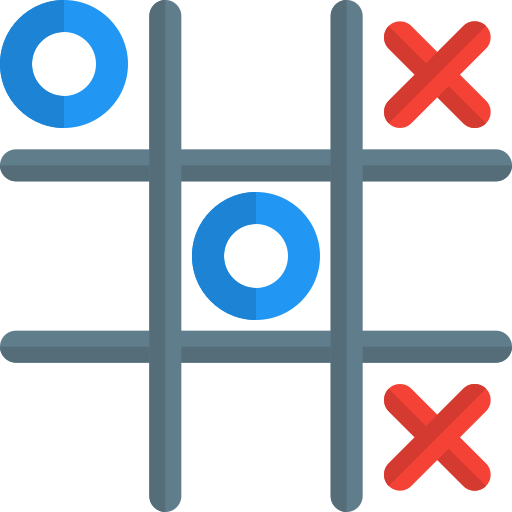
\includegraphics[width=0.05\textwidth,height=\textheight]{XsOs.png}
  needs to know where put the next {\textbf{X}} in order to win.
\item
  The computer of a self-driving car needs to know whether a particular
  patch of colours in the visual field is a person, so as to slow down
  the car and stop.
\item
  A rocket engineer needs to know, within two significant digits,
  \href{http://nasaphysics.cet.edu/escape-velocity.html}{how much is the
  velocity \(\sqrt{2\,G\,M/r\,}\)}, where
  \(G=6.67 \cdot 10^{-11}\,\mathrm{m^3\,s^{-2}\,kg^{-1}}\), and
  \(M = 5.97 \cdot 10^{24}\,\mathrm{kg}\) and
  \(r = 6.37 \cdot 10^{6}\,\mathrm{m}\) are the mass and radius of the
  Earth, in order to launch a rocket to the Moon.
\item
  We'd like to know whether the rolled die will show ⚅, so we can win a
  bet.
\item
  An
  \href{https://aerospaceamerica.aiaa.org/features/a-i-in-the-cockpit}{aircraft's
  autopilot system} needs to predict how much the
  \href{https://www.grc.nasa.gov/www/k-12/VirtualAero/BottleRocket/airplane/roll.html}{aircraft's
  roll} will change by increasing the right wing's
  \href{https://www.grc.nasa.gov/www/k-12/VirtualAero/BottleRocket/airplane/incline.html}{angle
  of attack} by 0.1~rad.
\item
  An archaeologist would like to know whether the fossil bone just dug
  out belonged to a Tyrannosaurus rex.
\item
  An automated system in an assembly line needs to predict whether an
  electric component of a widget will fail within the next two years.
\end{enumerate}

Note how each of these inferences boils down to determining whether some
sentences are true or false. In example 1. we want to know whether the
sentence \emph{``It rains today''} is true or not. In example 2. the
clinician wants to know which of the sentences \emph{``The patient has
pneumonia''}, \emph{``The patient has asthma''}, \emph{``The patient has
bronchitis''}, and so on, are true (several can be true at the same
time). In example 5. the rocket engineer wants to know which among the
sentences \emph{``The velocity is~~\(0.010\,\mathrm{m/s}\)''},
\emph{``The velocity is~~\(0.011\,\mathrm{m/s}\)''}, \ldots, \emph{``The
velocity is~~\(130\,\mathrm{m/s}\)''}, and so on, is true. The sentences
that underlie an inference can be extremely many and complex, and yet we
must have an idea of what they are (otherwise, do we really know what
our inference is about?).

\marginnote{\begin{footnotesize}

\begin{tcolorbox}[enhanced jigsaw, title=\textcolor{quarto-callout-tip-color}{\faLightbulb}\hspace{0.5em}{Exercise}, colbacktitle=quarto-callout-tip-color!10!white, coltitle=black, leftrule=.75mm, colback=white, rightrule=.15mm, opacitybacktitle=0.6, colframe=quarto-callout-tip-color-frame, toprule=.15mm, bottomtitle=1mm, bottomrule=.15mm, opacityback=0, toptitle=1mm, titlerule=0mm, breakable, arc=.35mm, left=2mm]

Try to identify which sentences underlie the other example inferences.

\end{tcolorbox}

\end{footnotesize}}

\hypertarget{certain-and-uncertain-inference}{%
\section{Certain and uncertain
inference}\label{certain-and-uncertain-inference}}

The example inferences above present very different levels of
difficulty.

Inferences 3. and 5. are special because they can actually be drawn
\emph{exactly}, that is, we really find out which of their underlying
sentences are true and false. In example 3. it is trivial that putting
the next {\textbf{X}} in the mid-right slot makes the X-player win. In
example 5. a couple of mathematical operations show that the sentence
\emph{``The velocity is \(11\,\mathrm{km/s}\)''} is true. When we can
obtain the data we want from the data we have by using
``only''\sidenote{\footnotesize ``Only'' in quotation marks because the logical
  analysis and operations leading to the answer can still be
  computationally very expensive.} logic and mathematical operations,
our inference is \emph{certain}, also called a ``deduction''; in these
notes we shall call it a \emph{truth inference}. But every deduction can
be basically drawn by repeatedly applying the rules of logic.

The other example inferences cannot be drawn exactly, in the sense that
we cannot know for sure whether all their underlying sentences are true
or false. But this doesn't mean that we cannot say anything whatsoever.
In example 6. we consider the sentence \emph{``The die shows ⚅''} to be
more likely false than true. In example 2. the clinician might be quite
sure about the disease, after observing the symptoms. On the other hand,
in example 1. we might really have no clue whether \emph{``It rains
today''} will turn out to be true or false. These inferences are
\emph{uncertain}. Certain inferences can be considered as a limit case
of uncertain ones, in which the uncertainty vanishes or is extremely
small.

To draw certain inferences, we follow the rules of Logic. What rules do
we follow to draw uncertain inferences?

\bookmarksetup{startatroot}

\hypertarget{truth-inference-and-probability-inference}{%
\chapter{Truth inference and probability
inference}\label{truth-inference-and-probability-inference}}

\hypertarget{logic-the-rules-for-certain-inference}{%
\section{Logic: the rules for certain
inference}\label{logic-the-rules-for-certain-inference}}

Consider the following trivial but certain inference: \[
\frac{
\textit{\small``My umbrella is either blue or red''}\quad
\textit{\small``My umbrella is not red''}
}{
\textit{\small``My umbrella is blue''}
}
\] Above the line we write the sentences representing the data we have.
Below the line we infer the information that supposedly interests us.

How could we draw this obvious inference? Which rules did we follow?

Logic is a huge field that formalizes and makes rigorous the rules that
a rational person or an artificial intelligence should use in drawing
certain inferences. We'll get a glimpse of it here, as a trampoline for
jumping towards our data-driven engineering problems.

\hypertarget{basic-sentences}{%
\subsection{Basic sentences}\label{basic-sentences}}

We start by writing down the \emph{basic}\sidenote{\footnotesize A more technical term
  is ``atomic''} sentences that constitute our data and that underlie
the inferences we want to draw. ``Basic'' in the sense that we will not
analyse these sentences into further sub-sentences. In the trivial
example above we identify two such sentences: \emph{``My umbrella is
blue''}, and \emph{``My umbrella is pink''}. Let's represent them by
symbols: \[
\begin{aligned}
b &\coloneqq \textit{\small``My umbrella is blue''}
\\
r &\coloneqq \textit{\small``My umbrella is red''}
\end{aligned}
\]

\hypertarget{connectives}{%
\subsection{Connectives}\label{connectives}}

You notice that we didn't consider \emph{``My umbrella is either blue or
red''} and \emph{``My umbrella is not red''} as basic sentences. These
sentences can indeed be expressed in terms of the basic sentences \(b\)
and \(r\). We consider one way or operation to change a sentence into
another related to it, and two ways or operations to combine two or more
sentences together. These operations are called ``connectives''. Our
natural language offer many more operations to combine sentences, but
these three turn out to be all we need in virtually all engineering
problems. The three connectives are:

\begin{description}
\tightlist
\item[Not: \(\lnot\)]
for example, \[
\lnot r = \textit{\small``My umbrella is not red''}
\]
\item[And: \(\land\)]
for example, \[
b \land r = \textit{\small``My umbrella is blue, and it is red''}
\]
\item[Or: \(\lor\)]
for example, \[
b \lor r = \textit{\small``My umbrella is blue, or it is red''}
\]
\end{description}

\begin{tcolorbox}[enhanced jigsaw, colframe=quarto-callout-warning-color-frame, toprule=.15mm, bottomrule=.15mm, arc=.35mm, opacityback=0, colback=white, rightrule=.15mm, breakable, leftrule=.75mm, left=2mm]
\begin{minipage}[t]{5.5mm}
\textcolor{quarto-callout-warning-color}{\faExclamationTriangle}
\end{minipage}%
\begin{minipage}[t]{\textwidth - 5.5mm}

\textbf{}\vspace{2mm}

Note some subtleties in

\end{minipage}%
\end{tcolorbox}

\hypertarget{truth-falsity-and-their-consistency}{%
\section{Truth, falsity, and their
consistency}\label{truth-falsity-and-their-consistency}}

\hypertarget{inferences-without-uncertainty-the-truth-calculus}{%
\section{Inferences without uncertainty: the truth
calculus}\label{inferences-without-uncertainty-the-truth-calculus}}

\hypertarget{making-room-for-uncertainty-plausibility-credibility-degree-of-belief-probability}{%
\section{\texorpdfstring{Making room for uncertainty:Plausibility,
credibility, degree of belief,
probability}{Making room for uncertainty: Plausibility, credibility, degree of belief, probability}}\label{making-room-for-uncertainty-plausibility-credibility-degree-of-belief-probability}}

\hypertarget{inferences-with-uncertainty-the-probability-calculus}{%
\section{Inferences with uncertainty: the probability
calculus}\label{inferences-with-uncertainty-the-probability-calculus}}

\hypertarget{the-three-fundamental-laws-of-inference}{%
\subsection{The Three Fundamental Laws of
inference}\label{the-three-fundamental-laws-of-inference}}

\begin{itemize}
\item
  \emph{Exercise: \href{The_Monty_Hall_problem-exercise.pdf}{Monty-Hall
  problem \& variations}}
\item
  \emph{Exercise: clinical test \& diagnosis}
\end{itemize}

\hypertarget{bayess-theorem}{%
\subsection{Bayes's theorem}\label{bayess-theorem}}

\hypertarget{common-points-of-certain-and-uncertain-inference}{%
\section{Common points of certain and uncertain
inference}\label{common-points-of-certain-and-uncertain-inference}}

\begin{quote}
\emph{No premises? No conclusions!}
\end{quote}

\bookmarksetup{startatroot}

\hypertarget{data-and-information}{%
\chapter{Data and information}\label{data-and-information}}

\hypertarget{kinds-of-data}{%
\section{Kinds of data}\label{kinds-of-data}}

\hypertarget{binary}{%
\subsection{Binary}\label{binary}}

\hypertarget{nominal}{%
\subsection{Nominal}\label{nominal}}

\hypertarget{ordinal}{%
\subsection{Ordinal}\label{ordinal}}

\hypertarget{continuous}{%
\subsection{Continuous}\label{continuous}}

\begin{itemize}
\item
  unbounded
\item
  bounded
\item
  censored
\end{itemize}

\hypertarget{complex-data}{%
\subsection{Complex data}\label{complex-data}}

2D, 3D, images, graphs, etc.

\hypertarget{soft-data}{%
\subsection{``Soft'' data}\label{soft-data}}

\begin{itemize}
\item
  orders of magnitude
\item
  physical bounds
\end{itemize}

\hypertarget{data-transformations}{%
\section{Data transformations}\label{data-transformations}}

\begin{itemize}
\item
  log
\item
  probit
\item
  logit
\end{itemize}

\bookmarksetup{startatroot}

\hypertarget{allocation-of-uncertainty-among-possible-data-values-probability-distributions}{%
\chapter{Allocation of uncertainty among possible data values:
probability
distributions}\label{allocation-of-uncertainty-among-possible-data-values-probability-distributions}}

\hypertarget{the-difference-between-statistics-and-probability-theory}{%
\section{The difference between Statistics and Probability
Theory}\label{the-difference-between-statistics-and-probability-theory}}

\emph{Statistics} is the study of collective properties of collections
of data. It does not imply that there is any uncertainty.

\emph{Probability theory} is the quantification and propagation of
uncertainty. It does not imply that we have collections of data.

\hypertarget{whats-distributed}{%
\section{What's ``distributed''?}\label{whats-distributed}}

Difference between distribution of probability and distribution of (a
collection of) data.

\hypertarget{distributions-of-probability}{%
\section{Distributions of
probability}\label{distributions-of-probability}}

\hypertarget{representations}{%
\subsection{Representations}\label{representations}}

\begin{itemize}
\item
  Density function
\item
  Histogram
\item
  Scatter plot
\end{itemize}

Behaviour of representations under transformations of data.

\hypertarget{summaries-of-distributions-of-probability}{%
\section{Summaries of distributions of
probability}\label{summaries-of-distributions-of-probability}}

\hypertarget{location}{%
\subsection{Location}\label{location}}

Median, mean

\hypertarget{dispersion-or-range}{%
\subsection{Dispersion or range}\label{dispersion-or-range}}

Quantiles \& quartiles, interquartile range, median absolute deviation,
standard deviation, half-range

\hypertarget{resolution}{%
\subsection{Resolution}\label{resolution}}

Differential entropy

\hypertarget{behaviour-of-summaries-under-transformations-of-data-and-errors-in-data}{%
\subsection{Behaviour of summaries under transformations of data and
errors in
data}\label{behaviour-of-summaries-under-transformations-of-data-and-errors-in-data}}

\hypertarget{outliers-and-out-of-population-data}{%
\section{Outliers and out-of-population
data}\label{outliers-and-out-of-population-data}}

(Warnings against tail-cutting and similar nonsense-practices)

\hypertarget{marginal-and-conditional-distributions-of-probability}{%
\section{Marginal and conditional distributions of
probability}\label{marginal-and-conditional-distributions-of-probability}}

\hypertarget{collecting-and-sampling-data}{%
\section{Collecting and sampling
data}\label{collecting-and-sampling-data}}

\hypertarget{representative-samples}{%
\subsection{``Representative'' samples}\label{representative-samples}}

Size of minimal representative sample = (2\^{}entropy)/precision

\begin{itemize}
\tightlist
\item
  \emph{Exercise: data with 14 binary variates, 10000 samples}
\end{itemize}

\hypertarget{unavoidable-sampling-biases}{%
\subsection{Unavoidable sampling
biases}\label{unavoidable-sampling-biases}}

In high dimensions, all datasets are outliers.

Data splits and cross-validation cannot correct sampling biases

\hypertarget{quirks-and-warnings-about-high-dimensional-data}{%
\section{Quirks and warnings about high-dimensional
data}\label{quirks-and-warnings-about-high-dimensional-data}}

\bookmarksetup{startatroot}

\hypertarget{making-decisions}{%
\chapter{Making decisions}\label{making-decisions}}

\hypertarget{decisions-possible-situations-and-consequences}{%
\section{Decisions, possible situations, and
consequences}\label{decisions-possible-situations-and-consequences}}

\hypertarget{gains-and-losses-utilities}{%
\section{Gains and losses: utilities}\label{gains-and-losses-utilities}}

\hypertarget{factors-that-enter-utility-quantification}{%
\subsection{Factors that enter utility
quantification}\label{factors-that-enter-utility-quantification}}

Utilities can rarely be assigned a priori.

\hypertarget{making-decisions-under-uncertainty-maximization-of-expected-utility}{%
\section{Making decisions under uncertainty: maximization of expected
utility}\label{making-decisions-under-uncertainty-maximization-of-expected-utility}}

\bookmarksetup{startatroot}

\hypertarget{the-most-general-inference-problem}{%
\chapter{The most general inference
problem}\label{the-most-general-inference-problem}}



\end{document}
